\documentclass{tufte-handout}
\usepackage{tikz}
\usepackage{mathtools}

\usetikzlibrary{shapes,arrows,matrix,fit,positioning,decorations.pathreplacing}
% Diagrams styles
\tikzstyle{block} = [draw=black, rectangle, minimum height=2.5em, minimum width=2em]
\tikzstyle{sum} = [draw=black, circle]
\tikzstyle{gain} = [draw=black, regular polygon, regular polygon sides=3, regular polygon rotate=90, minimum height=2.5em, minimum width=2em]
\tikzstyle{input} = [coordinate]
\tikzstyle{output} = [coordinate]
\tikzstyle{pinstyle} = [pin edge={to-,thin,black}]

\begin{document}
%\begin{tikzpicture}[auto,>=latex']
%	\coordinate (center);
%	\coordinate[at=(center.0), anchor=mid, shift=(62.05-90:0.6mm)] (pointA1);
%	\coordinate[at=(center.0), anchor=mid, shift=(153.3-90:1mm)] (pointB1);
%	\coordinate[at=(center.0), anchor=mid, shift=(260-90:1mm)] (pointC1);
%	
%	\coordinate[at=(pointA1.0), anchor=mid, shift=(0-90:15mm)] (pointA2);
%	\coordinate[at=(pointB1.0), anchor=mid, shift=(124.1-90:14.5mm)] (pointB2);
%	\coordinate[at=(pointC1.0), anchor=mid, shift=(180-90:15.5mm)] (pointC2);
%
%	\filldraw[fill=gray, draw=black] (pointA1) -- (pointA2) arc (0-90:124.1-90:15mm) -- cycle;
%	\filldraw[fill=white, draw=black] (pointB1) -- (pointB2) arc (124.1-90:180-91.5:15mm) -- cycle;
%	\filldraw[fill=gray, draw=black] (pointC1) -- (pointC2) arc (180-90:360-90:15.5mm) -- cycle;
%
%	\node[at=(pointA1.0), anchor=(0), shift=(-15:13mm)] {34\%};
%	\node[at=(pointB1.0), anchor=(0), shift=(40:13mm)] {16\%};
%	\node[at=(pointC1.0), anchor=(0), shift=(180:3mm)] {50\%};
%
%	\node[at=(pointA1.0), anchor=(180), shift=(-80:20mm), text width=2cm] {\scriptsize{2 or 3 buried person}};
%	\node[at=(pointB1.0), anchor=(180), shift=(80:20mm), text width=2cm] {\scriptsize{more than 3 buried person}};
%	\node[at=(pointC1.0), anchor=(180), shift=(140:29mm), text width=2cm] {\scriptsize{1 buried person}};
%
%\end{tikzpicture}
%
%\vspace{3cm}
%\begin{tikzpicture}[auto,node distance=1cm,>=latex']
%
%	\node[regular polygon, regular polygon sides=3, regular polygon rotate=180, draw, minimum height=1cm] (ant) {};
%	\draw (ant.north) -- (ant.south);
%	
%	\node[below of=ant] (input) {};
%\begin{scope}[node distance=4mm and 6mm]
%	\node[block, right=of input, minimum width=2.3cm, text width=2cm, align=center] (b1) {\scriptsize{Triple Antennas}};
%	\node[block, right=of b1, minimum width=2.3cm, text width=2cm, align=center] (b2) {\scriptsize{Frequency shift \\ Anti--alias filter}};
%	\node[block, below=of b2, minimum width=2.3cm, text width=2cm, align=center] (b3) {\scriptsize{A--D \\ Conversion}};
%	\node[block, below=of b3, fill=white, minimum width=2.3cm, text width=2cm, align=center] (b4) {\scriptsize{Digital Filter}};
%	\node[block, left=of b4, minimum width=2.3cm, text width=2cm, align=center] (b5) {\scriptsize{Signal \\ Detection}};
%	\node[block, left=of b5, minimum width=2.3cm, text width=2cm, align=center] (b6) {\scriptsize{H--field \\ Estimation}};
%\end{scope}
%
%	\draw[->] (ant.south) |- (b1) {};
%	\draw[->] (b1) -- (b2) {};
%	\draw[->] (b2) -- (b3) {};
%	\draw[->] (b3) -- (b4) {};
%	\draw[->] (b4) -- (b5) {};
%	\draw[->] (b5) -- (b6) {};
%	\node [at=(b3.0), anchor=(180), shift=(0:3mm)] (n1) {};
%	\node [at=(b3.0), anchor=(180), shift=(180:88mm)] (n2) {};
%	\draw [dashed] (n2) -- (b3) {};
%	\draw [dashed] (n1) -- (b3) {};
%
%	\node [at=(n2.0), anchor=(180), shift=(25:10mm)] (n1) {Analog};
%	\node [at=(n2.0), anchor=(180), shift=(-25:10mm)] (n1) {Digital};	
%\end{tikzpicture}
%
%\vspace{3cm}
%\begin{tikzpicture}[auto, node distance=2cm,>=latex']
%
%	\matrix [draw=white, row sep=0.1cm, column sep=1.5cm] {	
%	   	& \node [block, right, anchor=west, text width=1.5cm, minimum width=1.5cm] (levelD) {Level 3}; & \\
%		& \node [block, right,anchor=west, text width=1.8cm, minimum width=1.8cm] (levelC) {Level 2}; & \\
%	 	& \node [block, right,anchor=west, text width=2.1cm, minimum width=2.1cm] (levelB) {Level 1}; & \\
%		\node [input,right] (input) {}; & \node [block,anchor=west, text width=2.4cm, right, minimum width=2.4cm] (levelA) {Level 0}; & \node[output](output){} ; \\
% 	};
%
%	\draw [->] (input) -- node[below](mid) {Sensors} (levelA);
%	\draw [->] (mid) |- node {} (levelB);
%	\draw [->] (mid) |- node(midU) {} (levelC);
%	\draw [->] (mid) |- node (midUb)  {} (levelD);
%	\draw [->] (levelA) -- node[below] (midA) {Actuators} (output);
%	\draw [->] (levelB) -| node[pos=0.3] (midB) {} (midA);
%	\draw [->] (levelC) -| node[pos=0.3] (midC) {} (midB.south);
%	\draw [->] (levelD) -| node[pos=0.3] (midD) {} (midC.south);
%
%	\draw [->,dotted] (midUb.south) -- node  {} ++(0,0.8);
%	\draw [<-,dotted] (midD.south) -- node {} ++(0,0.8);
%\end{tikzpicture}
%\vspace{2cm}
%
%
%\begin{tikzpicture}[auto, node distance=2cm,>=latex']
%	\node[input] (input) {};
%	\node[block,right of=input] (perception) {Perception};
%	\node[block,right of=perception] (action) {Action};
%	\node[output, right of=action] (output) {};
%
%	\draw[->] (input) -- node[pos=0.2] {Sensors} (perception);
%	\draw[->] (perception) -- (action);
%	\draw[->] (action) -- node[pos=0.7] {Actuators} (output);
%\end{tikzpicture}
%
%\vspace{2cm}
%
%
%\begin{tikzpicture}[auto, node distance=1cm,>=latex']
%	\node [rectangle, draw=black, minimum width=6cm,minimum height=4.5cm] (envir) {};
%	\node [rectangle, draw=black, minimum width=4cm,minimum height=3.5cm] (body) at ++(0.75cm,-0.25cm) {};
%	\node [rectangle, draw=black, dashed, minimum width=2cm,minimum height=2cm] (body) at ++(1.5cm,-0.75cm) {};
%	\node [rectangle, fill=white] (situatedness) at ++(-1.25cm,-0.5cm) {$\underset{situatedness}{\longleftrightarrow}$};
%	\node [rectangle, fill=white] (embodiment) at ++(.5cm,-1.25cm) {$\underset{embodiment}{\longleftrightarrow}$};
%	\node [rectangle, fill=white, draw=black] at ++(-1.5cm,2.3cm) {\textbf{Environment}};
%	\node [rectangle, fill=white, draw=black] at ++(1.8cm,1.5cm) {\textbf{Agent}};
%	\node at(-0.6cm,1.1cm) {Body};
%	\node at(1.1cm,-0.1cm) {Mind};
%\end{tikzpicture}
%
%
%
%\vspace{2cm}
%\begin{tikzpicture}[auto, node distance=2.7cm,>=latex']
%	% EMULATION
%	\matrix[draw=black, row sep=0.1cm, column sep=0.2cm] (emulator) {
%	 \node {\scriptsize{Model}}; \\ 
%	 \node {\scriptsize{Hypothesis}};  \\
%	};
%	\node[above of=emulator] at ++(0,-1.8cm) {Emulator};
%
%	% GROUNDING
%	\matrix [draw=black,minimum width=4cm, minimum height=2.5cm, row sep=0.1cm, column sep=1cm, above of=emulator] (grounding) at ++(0,0cm) {	
%		& \node [block, right,anchor=west, minimum width=1cm ,minimum height=0.5cm] (levelC) {}; & \\
%	 	& \node [block, right,anchor=west, minimum width=1.25cm ,minimum height=0.5cm] (levelB) {}; & \\
%		\node [input,right] (input) {}; & \node [block,anchor=west, right, minimum width=1.5cm, minimum height=0.5cm] (levelA) {}; & \node[output](output){} ; \\
% 	};
%	\node[above of=grounding] at ++(0,1.5cm) {Grounding};
%
%	% EMULATOR
%	\node[block,below of=emulator] (environment) at ++(0,1.2cm) {\textbf{Environment}};
%
%
%	\draw [->] (input) -- node[below](mid) {} (levelA);
%	\draw [->] (mid) |- node (midK) {} (levelB);
%	\draw [->] (mid) |- node(midU) {} (levelC);
%	
%	\draw [->] (levelA) -- node[below] (midA) {} (output);
%	\draw [->] (levelB) -| node[pos=0.3] (midB) {} (midA);
%	\draw [->] (levelC) -| node[pos=0.3] (midC) {} (midB.south);
%
%
%	\draw [->,dotted] (mid) -- node  {} ++(0,1.8);
%	\draw [<-,dotted] (midC.south) -- node {} ++(0,0.5);
%
%	\node[right of=grounding] (gr) {};
%	\node[left of=grounding] (gl) {};
%
%	\draw [->] (emulator.west) -|  (gl.south) |- (grounding);
%	\draw [<-] (emulator.east) -|  (gr.south) |- (grounding);
%
%	\node[block,minimum width=6cm, minimum height=5.25cm,dashed] (agent) at ++(0,1.9cm) {};
%	\node[above of=agent] at ++(0,2cm) {\textbf{Agent}};
%
%	\draw [<-] (environment.east) -- ++(2cm,0) |- (grounding);
%	\draw [<-] (environment.west) -- ++(-2cm,0) |- (grounding);
%
%\end{tikzpicture}

\vspace{3cm}
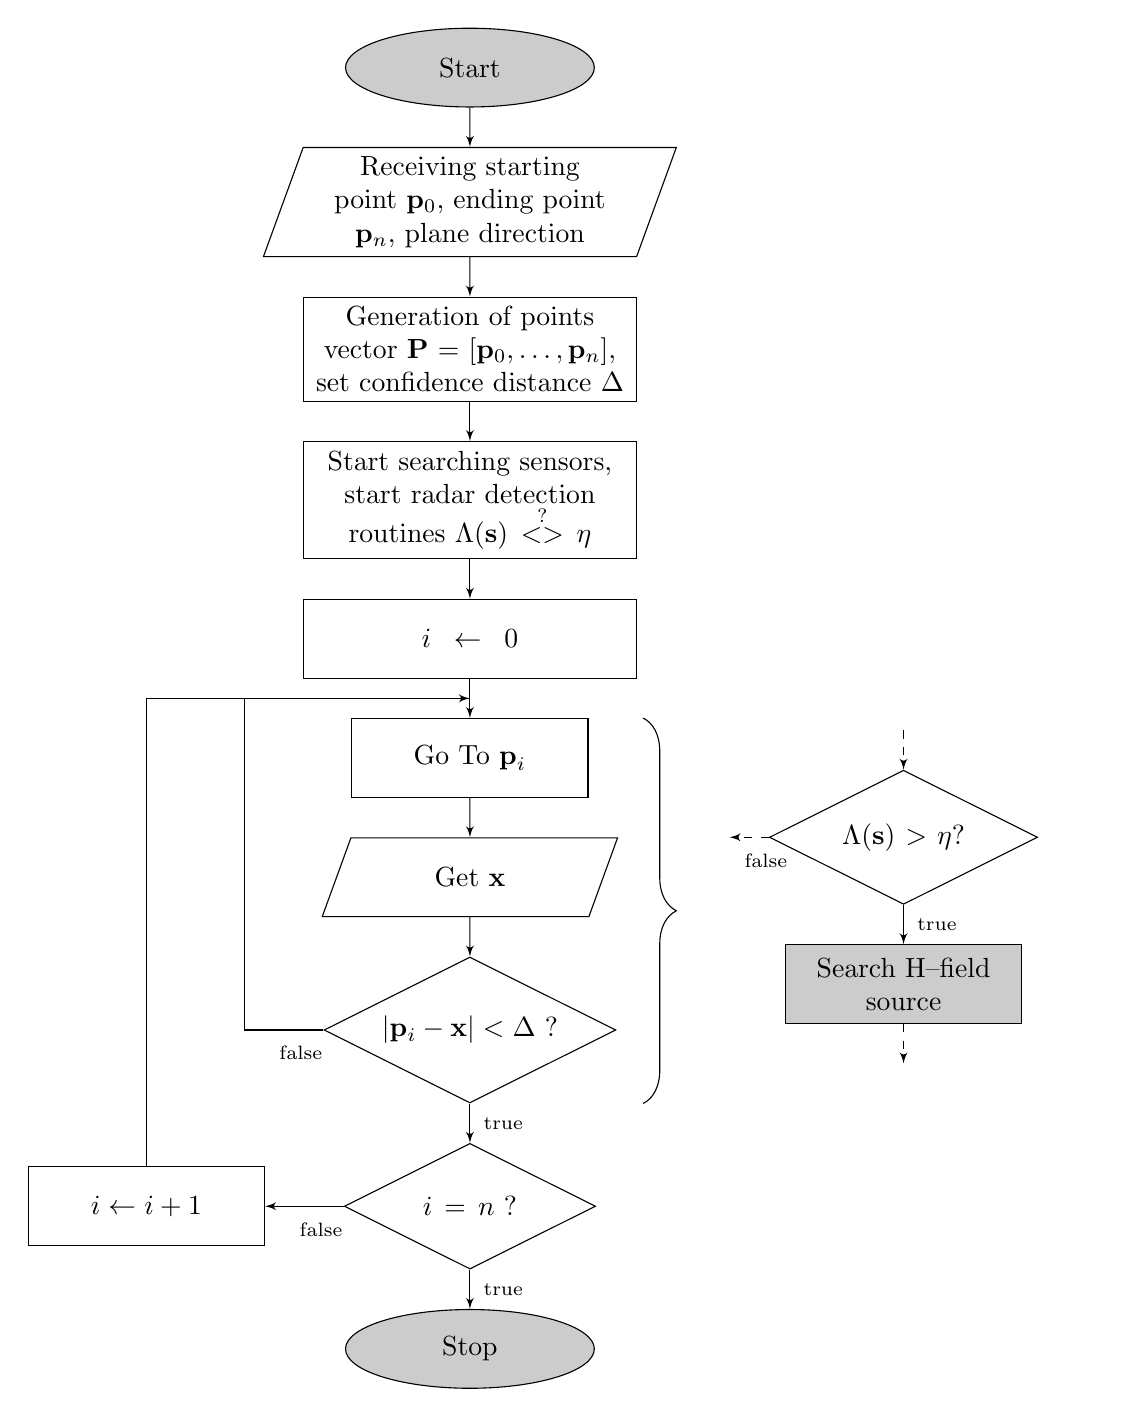
\begin{tikzpicture}[auto,node distance=0.5cm and 1cm, >=latex', minimum width=3cm, minimum height=1cm, text width=4cm, align=center]

	%\draw (0,0) ellipse (2cm and 1cm) node (start) {Start};
	%\draw

	\node [ellipse, draw, minimum width=2cm, text width=2cm, fill=gray!40] (start) {Start};
	\node [trapezium, draw, trapezium left angle=70,trapezium right angle=-70, below=of start] (inserimento) {Receiving starting point $\mathbf{p}_0$, ending point $\mathbf{p}_n$, plane direction};
	\node [rectangle, draw, below=of inserimento] (generazione_punti) {Generation of points vector $\mathbf{P} = [\mathbf{p}_0,\dots,\mathbf{p}_n]$, set confidence distance $\Delta$};
	\node [rectangle, draw, below=of generazione_punti] (abilita_ricerca) {Start searching sensors, start radar detection routines $\Lambda(\mathbf{s}) \overset{?}{<>} \eta$ };
	\node [rectangle, draw, below=of abilita_ricerca] (goto_start) {$i \leftarrow 0$};
	\node [rectangle, draw, below=of goto_start, text width=2cm] (select_point) {Go To $\textbf{p}_i$};
	\node [trapezium, draw, trapezium left angle=70, trapezium right angle=-70, below=of select_point,text width=1.2cm] (read_position) {Get $\mathbf{x}$};
	\node [diamond, draw, aspect=2, text width=2.3cm, below=of read_position] (distanza) {$\left| \mathbf{p}_i - \mathbf{x} \right| < \Delta$ ?};
	\node [diamond, draw, aspect=2, text width=2cm, below=of distanza] (lastpoint) {$i = n$ ?};
	\node [ellipse, draw, minimum width=2cm, text width=2cm, below=of lastpoint,fill=gray!40] (stop) {Stop};

	\node [rectangle,draw,left=of lastpoint, text width=1.5cm] (addone) { $i \leftarrow i+1$ };
	\coordinate [at=(select_point.north), shift=(0:22mm)] (braces_a);
	\coordinate [at=(distanza.south), shift=(0:22mm)] (braces_b);
	\draw [decorate,decoration={brace,amplitude=12pt}] (braces_a) -- (braces_b) {};

	\node [diamond, draw, aspect=2, text width=2cm, at=(read_position.north east), shift=(0:50mm)] (detection) {$\Lambda(\mathbf{s}) > \eta$?};
	\node [rectangle, draw,fill=gray!40, text width=2.5cm, below=of detection] (search) {Search \mbox{H--field} source};

	\coordinate [at=(detection.north), shift=(90:5mm)] (extraA);
	\coordinate [at=(search.south), shift=(270:5mm)] (extraB);
	\coordinate [at=(detection.west), shift=(180:5mm)] (extraC);
	\coordinate [at=(distanza.west), shift=(180:10mm)] (intraB);

	\draw [->] (start) -- (inserimento);
	\draw [->] (inserimento) -- (generazione_punti);
	\draw [->] (generazione_punti) -- (abilita_ricerca);
	\draw [->] (abilita_ricerca) -- (goto_start);
	\draw [->] (goto_start) -- coordinate[pos=0.5](intraA) (select_point);
	\draw [->] (select_point) -- (read_position);
	\draw [->] (read_position) -- (distanza);
	\draw [->] (distanza) -- node[shift=(0:-17mm)]{\scriptsize{true}} (lastpoint);
	\draw [->] (lastpoint) -- node[shift=(0:-17mm)]{\scriptsize{true}} (stop);
	\draw [->] (detection) -- node[shift=(0:-17mm)]{\scriptsize{true}} (search);
	\draw [->] (lastpoint) -- node[shift=(45:3mm)]{\scriptsize{false}} (addone);

	\draw [->,dashed] (extraA) -- (detection);
	\draw [->,dashed] (search) -- (extraB);
	\draw [->,dashed] (detection) -- node[shift=(45:3mm)]{\scriptsize{false}} (extraC);

	\draw [->] (addone) |- (intraA);
	\draw (distanza) -- node[shift=(45:3mm)]{\scriptsize{false}} (intraB) |- (intraA);

\end{tikzpicture}
\end{document}